\documentclass{article} % A4 paper and 11pt font size
\usepackage[T1]{fontenc} % Use 8-bit encoding that has 256 glyphs
\usepackage{mathpazo}

\usepackage[letterpaper, margin=1.25in]{geometry}
\usepackage{parskip}
\usepackage{setspace}
\usepackage{titlesec}
\titleformat{\section}[hang]{\normalfont\scshape\bfseries}{\thesection}{1em}{}
\titleformat{\subsection}[runin]{\normalfont\scshape}{\thesection}{1em}{}
\titlespacing{\section}{0pt}{15pt}{1em}[]

\usepackage[document]{ragged2e}

\usepackage{siunitx}
\usepackage{amsmath}
\usepackage{graphicx}
\usepackage{xcolor}
\usepackage{placeins}

\usepackage[style=apa,sortcites=true,sorting=nyt,backend=biber]{biblatex}
\addbibresource{ref.bib}

\usepackage{fancyhdr} % Custom headers and footers
\pagestyle{fancyplain} % Makes all pages in the document conform to the custom headers and footers
\fancyhead{} % No page header - if you want one, create it in the same way as the footers below
\fancyfoot[L]{} % Empty left footer
\fancyfoot[C]{} % Empty center footer
\fancyfoot[R]{\thepage} % Page numbering for right footer
\renewcommand{\headrulewidth}{0pt} % Remove header underlines
\renewcommand{\footrulewidth}{0pt} % Remove footer underlines
\setlength{\headheight}{13.6pt} % Customize the height of the header

\setlength\parindent{0pt} % Removes all indentation from paragraphs - comment this line for an assignment with lots of text

% ----------------------------------------------------------------------------------------
%	TITLE SECTION
% ----------------------------------------------------------------------------------------

\newcommand{\horrule}[1]{\rule{\linewidth}{#1}} % Create horizontal rule command with 1 argument of height

\title{
  \normalfont \normalsize
  \textsc{The University of British Columbia} \\ [25pt] % Your university, school and/or department name(s)
  \horrule{0.5pt} \\[0.4cm] % Thin top horizontal rule
  \huge BMEG 101 - Cellular and Molecular Bioengineering Project Assignment % The assignment title
  \horrule{2pt} \\[0.5cm] % Thick bottom horizontal rule
}

\author{Alex Koen \& Chloe Bolongaro} % Your name

\date{\normalsize \today} % Today's date or a custom date

\begin{document}

\maketitle % Print the title

\onehalfspacing

\begin{enumerate}
\item \textit{Design of the 1-dimensional cell culture system. Explain appropriate size and materials you will use, and provide a diagram of the set up.}

  Since the average mammalian cell is \SI{10}{\micro\m} in diameter, the tube will be \SI{10}{\milli\m} long to support one thousand cells in a row.

  Stem cell cultures are delicate, and depend on external support for cell survival and to allow for self-renewal. The 1-dimensional cell culture used in this project will be composed of a polycaprolactone outer structure, which has been shown to act effectively as a bioinert scaffold \parencite{bertucci2018biomaterial}. While it would be ideal to coat the scaffold with a complete extracellular matrix to promote cell attachment, the inner wall will be coated with fibronectin instead for simplicity and robustness.

  The tube will be maintained at a temperature of \SI{37}{\celsius} by controlling the ambient temperature around the tube. Furthermore, the tube will be filled with human platelet lysate to provide the cells with the ideal nutrients and pH they need to survive.

\item  \textit{Explain how you will provide BMP4 activation in just one edge of the tube.}

BMP4 activation will be provided in just one edge of the tube by pumping the ligand into the tube through a one-way valve. {\color{red}(expand)}
  
\item \textit{Calculate the decay length, $\lambda$ of the BMP4 concentration gradient}
  
  \begin{align*}
    \lambda &= \sqrt{\frac{D}{k}} \\
            &= \sqrt{\frac{\SI{1.2}{\micro\m^2\per\s}}{\SI{5.4e-5}{\per\s}}} \\
            &= \SI{149}{\micro\m} \\
  \end{align*}
\item Write differential equations for the dynamics of the BMP4 concentration and BMPR2 concentration.

  \textbf{Dynamics of BMP4:}
  
  \begin{align*}
    L &= L_0 e^{\frac{-x}{\lambda}} \\
    \intertext{This shows that the ligand concentration decreases exponentially along the tube. Now, taking the second derivative of $L$ with respect to $x$:}
    \frac{\partial L}{\partial x} &= \frac{-L_0}{\lambda}e^{\frac{-x}{\lambda}} \\
    \frac{\partial ^2L}{\partial x^2} &= \frac{L_0}{\lambda^2}e^{\frac{-x}{\lambda}}
                                        \intertext{Given $\frac{\partial L }{\partial t} = D\frac{\partial^2 L}{\partial x^2}-kL+\nu$ (Fick's second law with a sink and a source):}
                                        \frac{\partial L}{\partial t} &= \frac{DL_0}{\lambda^2}e^{\frac{-x}{\lambda}}-kL_0e^{\frac{-x}{\lambda}} + \nu \\
      &= L_0e^{\frac{-x}{\lambda}}\left(\frac{D}{\lambda^2} -k \right) + \nu
  \end{align*}
  
  \textbf{Dynamics of BMPR2:}

  It is known that $R$ is produced linearly proportional to [BMP4] with proportionality constant $\alpha$ and degraded with rate constant $K_R$.

  \begin{align*}
    \frac{dR}{dt} &= \alpha L-k_R R \\
    \intertext{and given}
    L &= L_0 e^{\frac{-x}{\lambda}} \\
    \frac{dR}{dt} &= \alpha L_0 e^{\frac{-x}{\lambda}} -k_R R \\
  \end{align*}

\item \textit{Find solutions for ligand and receptor equations in steady state.}

  $L_0=\SI{2}{\nano\g\per\micro\m}$

  $\alpha = \SI{5e-3}{\per\s}$

  $k_R= \SI{10e-3}{\per\s}$


  \textbf{Solution for ligand equation in steady-state:}

  In steady state, $\frac{\partial L}{\partial t} = 0$  

  \begin{align*}
    0 &= L_0e^{\frac{-x}{\lambda}}\left(\frac{D}{\lambda^2} -k \right) + \nu \\
    \nu &= L_0e^{\frac{-x}{\lambda}}\left(k - \frac{D}{\lambda^2} \right) \\
    \nu &= \SI{2}{\nano\g\per\micro\m}e^{\frac{-x}{149}} \left (\SI{5.4e-5}{\per\s} - \frac{\SI{1.2}{\micro\m^2\per\s}}{(\SI{149}{\micro\m})^2} \right ) \\
    \nu &= 0 \\
    \intertext{Additionally, since $k - \frac{D}{\lambda^2}=0$ it can be inferred that:}
    \frac{\partial L}{\partial t} &= \nu \\
    \intertext{and if the source is held constant:}
    \int \frac{\partial L}{\partial t}~dt&=\nu \int dt \\ 
    \Delta L &= \nu \Delta t
  \end{align*}

  This makes sense---the only way for the ligand concentration to be constant over time is if there \emph{is no} source of ligands. Also note that the rate of ligand diffusion is \emph{equal} to its effective degradation rate, given by $kL$. Consequently, the change in ligand concentration over time is independent of $x$ and determined solely by the source.
  

  \textbf{Solution for receptor equation in steady state:}

  \begin{align*}
    \frac{dR}{dt} &= \alpha L_0 e^{\frac{-x}{\lambda}} -k_R R \\
    0 &= \alpha L_0 e^{\frac{-x}{\lambda}} -k_R R \\
    R &= \frac{\alpha}{k_R} L_0e^{\frac{-x}{\lambda}} \\
    \intertext{at the end of the tube ($x=0$):}
    R &= \frac{\alpha}{k_R}L_0 \\
                  &= \frac{\SI{5e-3}{\per\s}}{\SI{10e-3}{\per\s}} \SI{2}{\nano\gram\per\micro\m} \\
                  &= \SI{1}{\nano\g\per\micro\m}
  \end{align*}
  
\item \textit{Considering the association constant $K_a$, calculate the concentration of the ligand-receptor complex in steady state at the distance from the source $x=\lambda$:}

  \begin{align*}
    K_a &= \frac{K_{on}}{K_{off}} \\
    [RL] &= K_a[R][L] \\
    \intertext{$L$ at $x=\lambda$:}
    L &= \frac{L_0}{e} \\ 
        &= \frac{\SI{2}{\nano\g\per\micro\m}}{e} \\
        &= \SI{0.74}{\nano\g\per\micro\m} \\
    \intertext{$R$ at $x=\lambda$:}
    R &= \frac{\alpha L}{k_R} \\
        &= \frac{\SI{5e-3}{\per\s}\cdot \SI{0.74}{\nano\g\per\micro\m}}{\SI{10e-3}{\per\s}} \quad \text{(from above)} \\
        &= \SI{0.37}{\nano\g\per\micro\m}
          \intertext{It follows that:}
          [RL] &= K_a\cdot\SI{0.74}{\nano\g\per\micro\m}\cdot\SI{0.37}{\nano\g\per\micro\m} \\
        &= \SI{0.27}{\nano\g^2\per\micro\m^2}\cdot K_a
  \end{align*}

  The concentration of the ligand-receptor complex $RL$--- subsequently denoted $C$---at $x=\lambda$ is therefore dependant on the association constant $K_a$.
  \item \textit{Design a network motif that can satisy the BRA+/SOX2 pattern for different concentration of the ligand-receptor complex. Provide a sketch of the network, and explain the underlying logic. In a Boolean logic approach, provide a simulation showing the time series of the Boolean dynamics.}

    \textbf{SOX2:}
    SOX2 is a transcription factor that plays a key role in maintaining the pluripotency of undifferentiated neural stem cells. Its principal function is to regulate the expression of other transcription factors, including Oct4, which is critically important in the self-renewal of stem cells \parencite{chambers2009transcriptional}.

    \textbf{BRA:} Brachyury, on the other hand, is another transcription factor coded by the gene TBXT that, when expressed, activates several genes important for cellular differentiation. Since BRA is expressed when a sufficient concentration of BMP4 binds with the BMPR2 receptor, it is expected that these cells will differentiate while those exposed to a lower BMP4 concentration will maintain pluripotency.

    \FloatBarrier
    \begin{figure}[h]
      \centering
      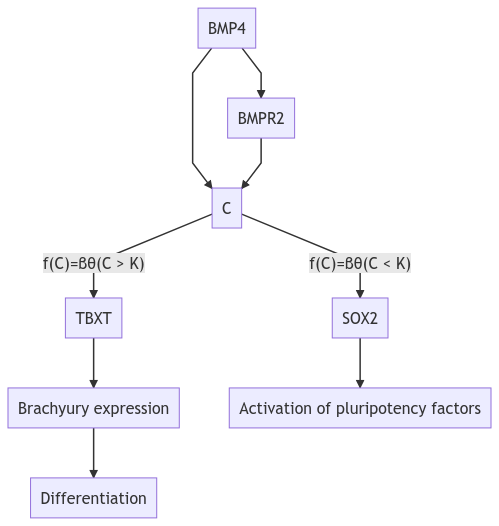
\includegraphics[width=0.6\textwidth]{motif}
      \caption{Network motif satisfying the pattern of BRA+/SOX2 interaction for different concentrations of the ligand-receptor complex.}
      \label{fig:motif}
    \end{figure} 
    \FloatBarrier

    In the network motif displayed in Figure \ref{fig:motif}, the concentration of the ligand-receptor complex $C$ is positively regulated by both the concentrations of BMP4 and BMPR2---which is itself regulated by the concentration of BMP4. When the concentration of the ligand-receptor complex exceeds the threshold value $K$ (at $x=\lambda$), expression of the TBXT gene turned on, modelled by the logic approximation $f(C)=\beta \theta (C > K)$, where $\beta$ is the maximal transcription rate and $\theta$ is either 0 or 1 depending on the result of the logic expression in parenthesis. When expressed, TBXT produces the brachyury transcription factor which in turns regulated other genes and eventually leads to cellular differentiation.

    Conversely, when the concentration of the ligand-receptor complex is less than the threshold value $K$, the cells remain SOX2 positive, and pluripotency is maintained.

    \FloatBarrier
    \begin{figure}[h]
      \centering
      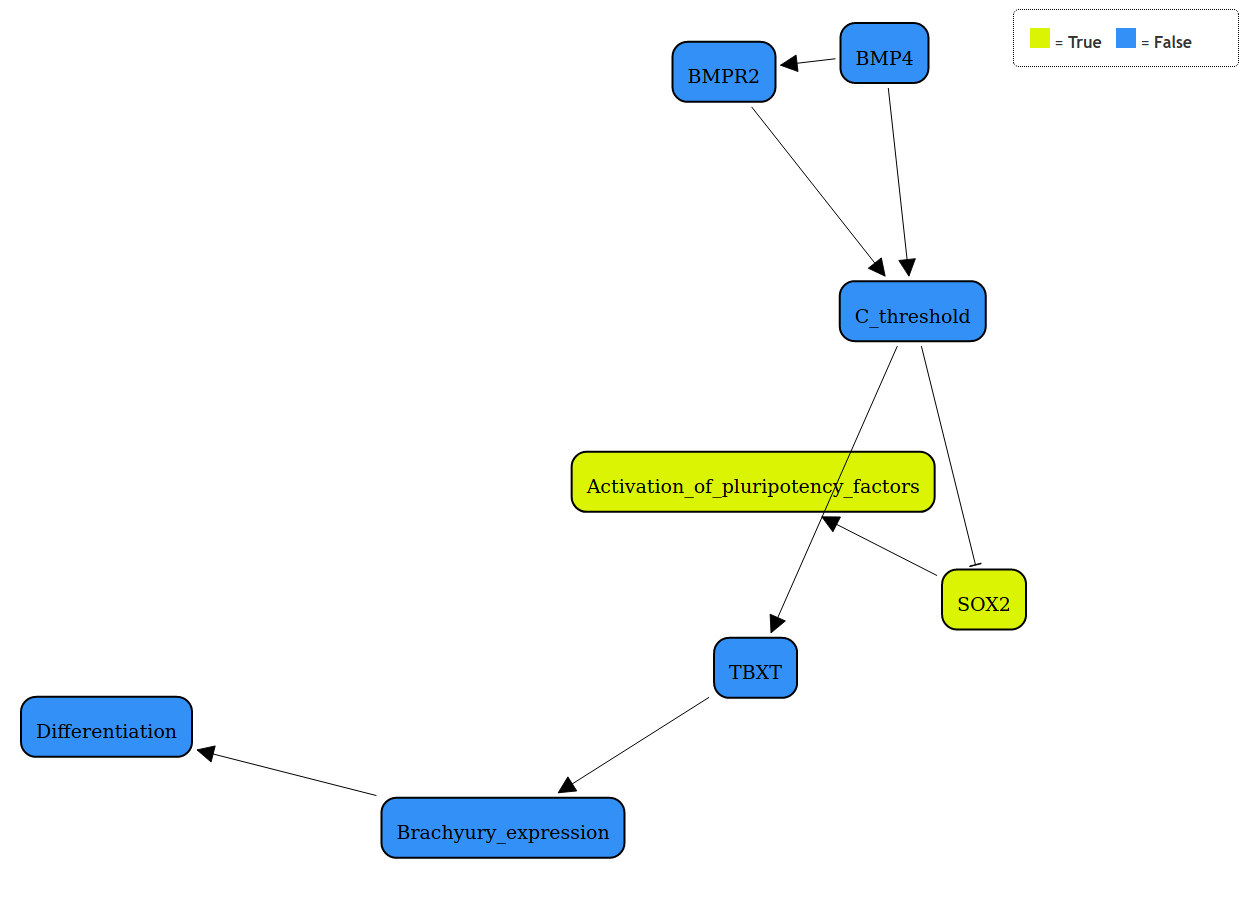
\includegraphics[width=0.8\textwidth]{bool1}
      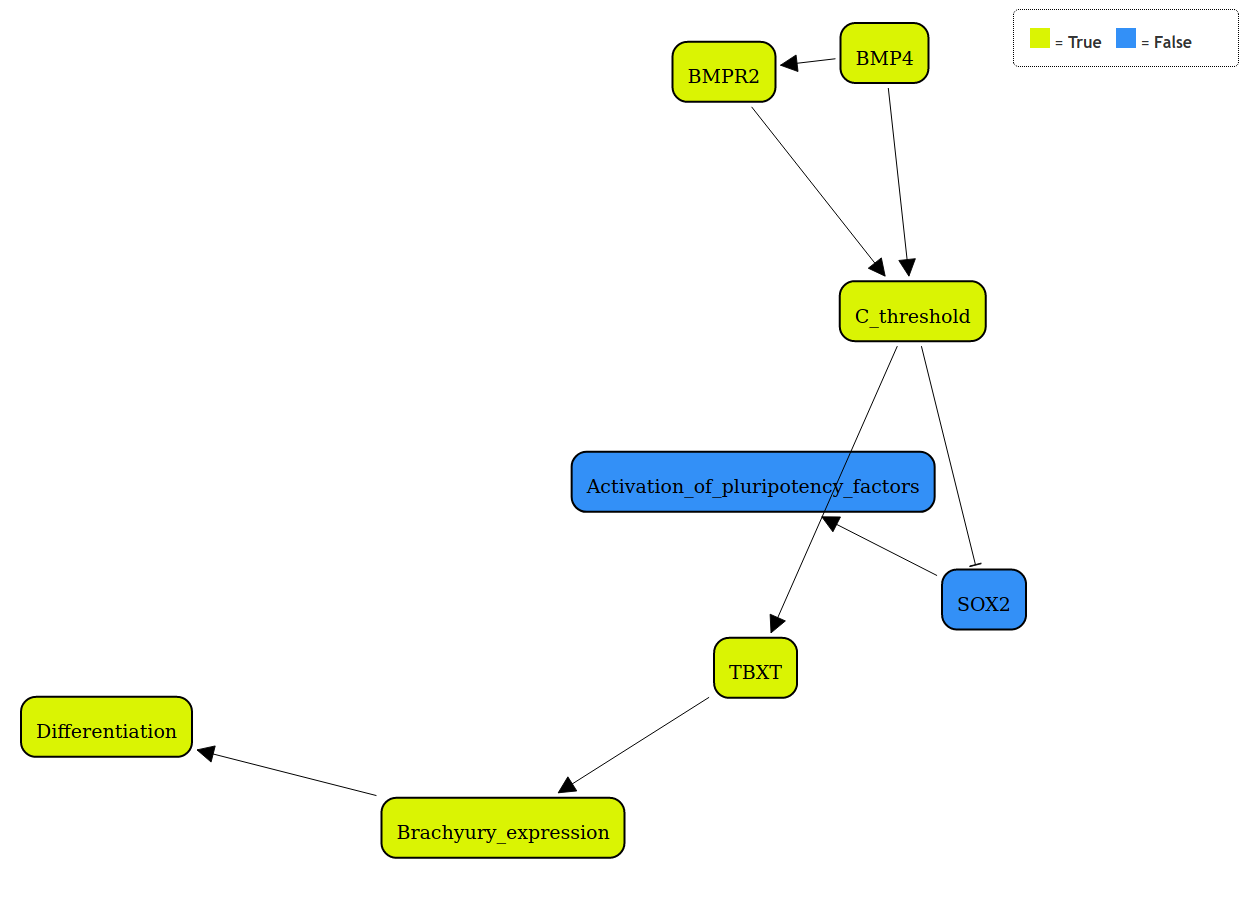
\includegraphics[width=0.8\textwidth]{bool2}
      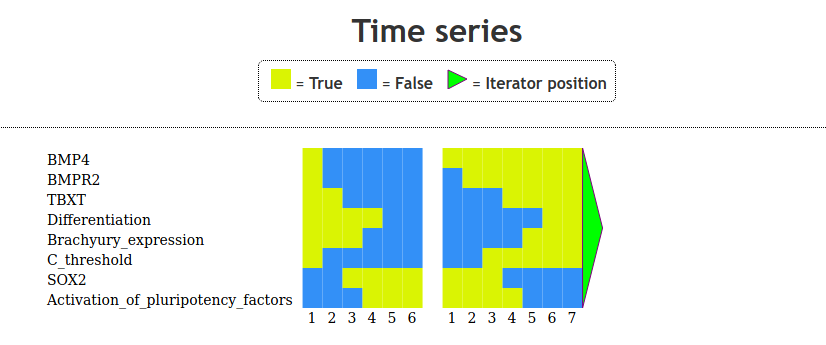
\includegraphics[width=0.8\textwidth]{time}
      \caption{Simulation of the given network motif using BooleSim. The time series shows the response of the above nodes to a change in BMP4 concentration.}
      \label{fig:bool1}
    \end{figure}
    \FloatBarrier

\item \textit{Discuss how you would build this network motif experimentally, which technology you would apply and why.}


  
\item \textit{Discuss how you would modify the size of the BRA+ region.}

  Note that the size of the BRA+ region is dependant  on two factors: the value of $\lambda$ and the value of $K_a$. At $x=\lambda$, the concentration of $C$ will always be the threshold value $\SI{0.27}{\nano\g^2\per\micro\m^2}\cdot K_a$, assuming $L_0$ is fixed. Therefore, by increasing or decreasing $\lambda$, the size of the BRA+ region will increase or decrease accordingly.

  $\lambda$ itself is dependant on two factors: the diffusion coefficient $D$ and the effective degradation rate $k$. If $D$ were to be increased, say by increasing the temperature, $\lambda$ would also increase. This is impractical, however, since the cells depend on a constant temperature of \SI{37}{\celsius} for survival. Therefore, one must decrease $k$ to increase $\lambda$.
  
\item \textit{Discuss how therapeutics can benefit from a precise control of differentiation patterns.}

  Therapeutics can benefit from precise control of differentiation patterns because such control would allow them to genetically engineer tissues and organs with specific cell types in a predetermined configuration. Currently, there are few stem cell therapies on the market because of risk associated with controlling their differentiation. For example, in a recent case autologous hematopoietic stem cells were injected into the kidneys of a patients with renal failure resulted in tumour growth \parencite{marks2017clarifying}. While most such cases are a result of illegitimate treatment, the technology is not yet at the point where it is safe to perform these treatments in a clinical setting.
\end{enumerate}

% \printbibliography

\end{document}

\implies
%%% Local Variables:
%%% mode: latex
%%% TeX-engine: xetex
%%% End:

% LocalWords:  pluripotency
